% --- [ Middle-end Components ] ------------------------------------------------

% <howto>
% * more detailed design of individual components (design)

% <howto>
% * The intention is that the design should be detailed enough to provide a good guide for actual coding, including details of any particular algorithms to be used.

\subsection{Middle-end Components}

% TODO: Visualize the dependency graph of the "restructure" tool and describe in detail what input it expects and what output it produces.

% TODO: Write about. Input and output LLVM IR to operate well with components written in other languages. Output LLVM IR with information about high-level control structures stored in the basic block names or in metadata.

% TODO: Mention package division.

% TODO: Rewrite and clarify.

The middle-end is responsible for lifting the LLVM IR to a high-level representation through a series of decompilation passes. The \texttt{ll2dot} tool generates a CFG (in the DOT file format) for each function of a given LLVM IR input file. The \texttt{restructure} tool searches for subgraph isomorphisms of control flow primitives in a given CFG. Once located the nodes identified subgraph are merged into a single node which is labeled with the high-level control flow primitive. Successive iterations continue to simplify the CFG until only one node is left, at which point the high-level control flow primitive has been recovered. Should the \texttt{restructure} tool fail to reduce the graph into a single node, the graph is considered irreducible with regards to the supported high-level control flow primitives. The interaction between the front-end, the \texttt{ll2dot} and \texttt{restructure} tools of the middle-end and the back-end is illustrated in figure \ref{fig:middle-end}.

% TODO: Write about the choice of subgraph isomorphism search algorithm. The
% properties of the control flow graph allows us to optimize.
%
% \cite{subgraph_isomorphism_algorithms}

\begin{figure}[htbp]
	\begin{center}
		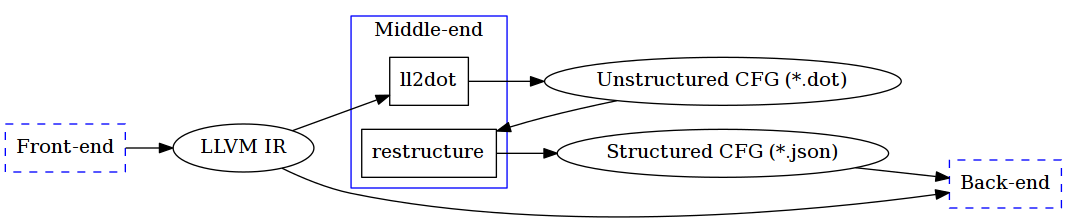
\includegraphics[width=\textwidth]{inc/middle-end.png}
		\caption{foo}
		\label{fig:middle-end}
	\end{center}
\end{figure}
